% \subsection {Algorithm Overview}

\begin{figure}
\begin{center}
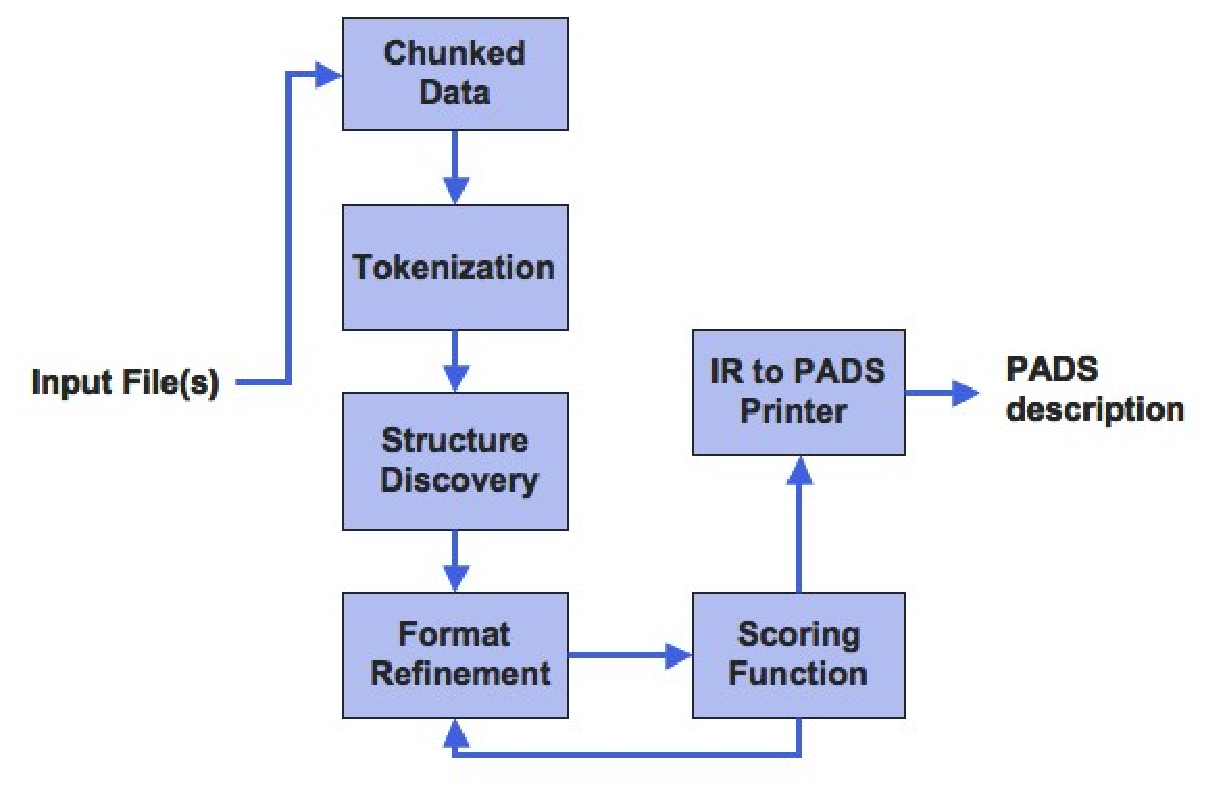
\epsfig{file=archi.eps, width=\columnwidth}
\caption{Architecture of the automatic tool generation engine}
\vspace*{-5mm}
\label{fig-archi}
\end{center}
\end{figure}

Figure \ref{fig-archi} gives an overview of our automatic
tool generation architecture. The process of generating a new
suite of data processing tools 
begins with raw data, shown in blue at the top left.  The
raw data is first piped into our format inference engine
(circumscribed by dotted lines in the picture).  The
format inference engine is implemented as a series of phases that 
eventually produce a syntactically correct \pads{} description
for the data.  Next, the generated \pads{} description is fed into the 
\pads{} compiler.  The compiler generates libraries that are linked to generic
programs for various tasks including a data analysis tool
({\em a.k.a.,} the {\em accumulator}) and an ad-hoc-to-\xml{} translator.
At this point, the user can apply these generated tools to their original 
raw data, or to other data with the same format.  

The following subsections describe the main components of the
inference algorithm in more detail, including chunking and
tokenization, the structure discovery phase, the information-theoretic
scoring function and the structure refinement phase.  We also
illustrate the action of each phase on our running examples and
present the final end products.

\subsection{Chunking and Tokenization}

The input data, which we also refer to as the {\em training set}, is first
divided into {\em chunks} as specified by the user.  Intuitively, a chunk
is a unit of repetition in the data source.  It is primarily by analyzing
a large number of repeated syntax elements that we are able to infer a usable
description for a data source.  Our tool currently supports
chunking on a line-by-line basis as well as on a file-by-file basis.  

Each chunk is broken down into a series of {\em simple tokens} by a lexer.
Each simple token can be a punctuation symbol, a number, a date, a time, or a
number of other basic items.  Every simple token type has a corresponding
base type in the \ir{}, though the converse is not true -- there are a
number of base types that are not used as tokens.  Nevertheless, since
simple tokens have a very close correspondence with base types,
we often use the word {\em token} interchangeably with {\em base type}.
  
Parenthetical syntax including quotation marks, curly braces, square brackets,
parentheses and \xml{} tags
often provides very important hints about the structure
of an ad hoc data file.  Therefore, whenever the lexer encounters 
a corresponding pair of parentheses, it 
creates what we call a {\em meta-token}, which is a single token that
represents the pair of parentheses and all simple tokens 
within.\footnote{If parenthetical elements
are not well-nested, the meta-tokens are discarded and replaced with
ordinary sequences of simple tokens.}  For example, in Crashreporter.log,
the syntax \cd{[2164]} will form the meta-token we write \cd{[*]} as
opposed to the three simple tokens \cd{[}, \cd{Pint}, and \cd{]}.  Meta-tokens
do not stay intact throughout the inference procedure:  As the structure 
discovery algorithm encounters each meta-token, it is cracked open and its 
underlying structure is analyzed.

Our learning system has a default tokenization scheme skewed toward systems
data, but users may specify a different scheme for their own domain
through a configuration file.  For example, computational biologists
may want to add DNA strings {\tt CATTGTT...} to the default tokenization 
scheme.  The configuration file is essentially
a list of name-regular expressions pairs.  The system uses the 
file to generate part of the system's lexer, a
collection of new \ir{} base types, and a series of type 
definitions that are incorporated into the final \pads{} specification.  

%% After tokenization, the algorithm enters the {\em structure discovery} 
%% phase.  This phase uses a top-down, divide-and-conquer
%% scheme to guess an approximate, initial format for the data.
%% To assess the quality of this initial approximation, the
%% algorithm computes an information-theoretic {\em score} for the
%% structure.  This score is used in the next phase to guide
%% {\em rewriting rules} that iteratively refine the format.  

%% Once the format has been refined to the extent possible, the resulting
%% \ir{} is printed in \pads{} syntax.  Template programs that use the
%% new description, including the \xml{}-converter, a simple
%% statistics tool we call the {\em accumulator}, a database tool
%% based on Oetiker's RRDTool~\cite{rrdtool}, and the \padx{}
%% query engine, are also all generated at this point.  Hence, starting
%% with data alone, our end-to-end algorithm quickly generates an entire suite
%% of fully functional data processing tools, ready to use at the command line.



% \begin{figure}
% \begin{verbatim}
% def triplet [0-9]{1,3}
% def doublet [0-9]{1,2}
% def hexdoub [0-9a-fA-F]{2}
% ...
% exp Pemail {str1}@{hostname}
% exp Pmac   ({hexdoub}(: | \-)){5}{hexdoub}
% exp PbXML  \<([a-zA-Z])+\>
% exp PeXML  \<\/[^>]+\>
% \end{verbatim}
% \caption{Tiny fragment of the default configuration file. 
% The configuration command {\tt exp} specifies the definition on that
% line should be  ``exported'' to
% the learning tool whereas command {\tt def} implies the definition
% is local and used only in other {\tt exp} or {\tt def} in the
% configuration file.}
% \label {fig:configfile}
% \end{figure}

%% 




%% \begin{figure}
%% \begin{center}
%% \begin{tabular}{|l|l|}
%% \hline
%% Name   &  Description               \\ \hline\hline
%% Pint  &   Integer \\ 
%% Palpha & Alpha-numeric string including '$\_$' and '$-$' \\
%% Pip & IP address \\
%% Pemail & Email address \\
%% Pmac & Mac address \\
%% Pdate & Simple date format \\
%% Ptime & Simple time format \\
%% Ppath & File system path \\
%% Phostname & Hostname \\
%% Purl  & URL \\
%% PbXML & Beginning XML tag \\
%% PeXML & Ending XML tag \\
%% Pother & Punctuation character \\\hline
%% \end{tabular}

%% \caption{Basic token types in default configuration.}
%% \label{figure:base-types}
%% \end{center}
%% \end{figure}
 



%%     *  mention system parameterization for multiple tokenizations for different domains
%%     * mention current skew towards systems data
%%     * ignore problems in this section -- save that for discussion/future work section
%%     * mention stream of tokens generated for running example 

\subsection {Structure Discovery}

Given a collection of tokenized chunks, the goal of the structure
discovery phase is to find a candidate description ``nearby'' a good
final solution.  In a later phase of the algorithm, the rewriting rules 
analyze, refine
and transform the candidate to produce that final solution.  The
high-level structure of the algorithm we use to discover candidate
descriptions was inspired by the work of Arasu and
Garcia-Molina on information extraction from web pages~\cite{arasu+:sigmod03}.
However, the context, goals and algorithmic details involved in our
work are entirely different.

%However, the details are
%entirely different as Arasu's algorithm operates over well-formed
%\html{} trees whereas our work focuses on the mucky world of ad hoc
%data.

\paragraph*{Structure Discovery Basics.}
Our algorithm operates by analyzing the collection of tokenized chunks
and guessing what the top-level type constructor is.  Based on this guess,
it will partition the chunks and recursively analyze each partition
to determine what the component types are.
Figure~\ref{fig:structure-discovery} presents an outline of how the
overall procedure operates.  The \cd{oracle} function,
whose implementation we leave hidden for now,
does most of the hard work in the algorithm by conjuring up 
one of four different sorts of prophecies.  

The \cd{BaseProphecy} simply reports that the top-level type
constructor is some specified base type.

The \cd{StructProphecy} specifies that the top-level description is a
struct.  In addition, if the struct is to have $k$ fields then the
\cd{StructProphecy} will carry a list (call it \cd{css}) with $k$
elements.  The $i^{\mathrm{th}}$ element in the list is a set of
chunks used recursively to discover the type of the $i^{\mathrm{th}}$
field of the struct.  These sets of chunks are derived from the
original input to the oracle function. More specifically, if the
oracle guesses there will be $k$ fields in the struct, then each original
chunk is partitioned into $k$ pieces. The $i^{\mathrm{th}}$ piece of
each original chunk is used to infer the $i^{\mathrm{th}}$ field of
the struct.

The \cd{ArrayProphecy} specifies that the top-level structure will
involve an array.  However, at this point in the inference algorithm,
predicting exactly where an array begins and ends is difficult, even
for the magical oracle.  Consequently, the algorithm actually
generates a three-field struct, where the first field allows for slop
prior to beginning the array, the middle field is the array itself,
and the last field allows for slop after the array is over.  If this
slop turns out to be unnecessary, the rewriting rules will clean up
the mess in the next phase.

Finally, the \cd{UnionProphecy} specifies that the top-level structure
will involve a union type.  Like a \cd{StructProphecy}, the
\cd{UnionProphecy} carries a \cd{chunks list} with it and each element
of the list is used recursively to infer a branch of the union.
Merging all elements of the list will result in the original input.
Intuitively, recursive partitioning of union chunks is done
``horizontally'' or as recursive partitioning of struct chunks is done
``vertically.''

As an example, recall the Crashreporter.log data presented in
Figure~\ref{fig:example}.  After tokenization, assuming a chunk is
a line of data, the two chunks from the example contain the following 
token sequences (recall \cd{[*]} and \cd{(*)} are meta-tokens encapsulating
everything within the respective parens):
{\small
\begin{verbatim}
Pdate ' ' Ptime ' ' Pint ' ' Palpha [*] ':' ...
'-' ' ' Palpha [*] ':' ' ' Palpha (*) ' ' ...
\end{verbatim}
}
\noindent
Given these token sequences, 
our oracle will guess that the top-level type constructor is a struct 
with three fields and divide up our original chunks into three sets
as follows.
{\small
\begin{verbatim}
Pdate ' ' Ptime ' ' Pint ' ' Palpha        (set 1)       
'-' ' ' Palpha 

[*]                                        (set 2)       
[*]

':' ...                                    (set 3)       
':' ' ' Palpha (*) ' ' ...
\end{verbatim}
}
\noindent
On recursive analysis of set 1, the oracle again suggests a struct is the top-level structure,
generating two more sets of chunks: 
{\small
\begin{verbatim}
Pdate ' ' Ptime ' ' Pint ' '               (set 4)       
'-' ' '

Palpha                                     (set 5)       
Palpha 
\end{verbatim}
}
\noindent
Now, since every chunk in set 5 contains exactly one base type
token, the recursion naturally bottoms out with the oracle claiming it has
found the base type \cd{Palpha}.  On the other hand, when analyzing set 4, 
the oracle detects insufficient commonality between chunks and decides
the top-most type constructor must be a union. It partitions set 4 into
two more sets, with each group containing only 1 chunk (either
\{\cd{Pdate ' ' ...}\} or \{\cd{'-' ' '}\}).  The first set is analyzed to 
determine the type of the first branch of the union and the second set 
is analyzed to determine the second branch of the union.
With no variation in either branch,
the algorithm quickly discovers an accurate type for each.

Backing out of the recursion, having completely discovered the
type of the data in set 1, we turn our attention to set 2.
On recursive analysis of this set, the meta-tokens are cracked open
and this piece of the data is recursively identified as having the type 
\cd{struct \{'['; Pint; ']';\}}.  Analysis of Set 3 proceeds in a similar 
fashion to the others.

%% The types $T_0$, $T_1$, $T_2$ and $T_3$ are not yet known -- they will
%% be constructed recursively.  $T_0$ is constructed by recursively applying
%% the discovery procedure to the data in the chunks that precedes
%% the first occurrence of \cd{Pdate}.  In this case, there is no such
%% data, so the inference procedure returns the trivial type \cd{Pempty} for
%% $T_0$.  $T_1$ is constructed by applying discovery to the data between
%% \cd{Pdate} and \cd{Ptime}.  Each chunk contains one token in this case,
%% the space token.  Hence the discovery procedure easily decides
%% $T_1$ is \cd{' '}. $T_2$ is discovered by recursively analyzing the following
%% two chunks.
%% {\small
%% \begin{verbatim}
%%    ' ' Pint ' ' Palpha '[' Pint ']' 
%%    ' ' Pint ' ' Palpha '[' Pint ']'
%% \end{verbatim}
%% }
%% \noindent
%% Finally, the structure of $T_3$ is discovered by recursively analyzing 
%% all data following the ':' token.

As a second example, consider the Sirius data from Figure~\ref{fig:example}.
Here the chunks have the following structure:
{\small
\begin{verbatim}
   Pint '|' Pint '|' ... '|' Pint '|' Pint
   Pint '|' Pint '|' ... '|' Palpha Pint '|' Pint
\end{verbatim}
}
\noindent
In this case, our algorithm guesses that the top-level structure involves
an array and hence partions the data into sets of chunks for the
array preamble, the array itself, and the array postamble.  The
preamble chunks all have the form \{\cd{Pint '|'}\} and the
postamble chunks all have the form \{\cd{Pint}\}, so their 
types easily discovered.  The algorithm discovers the type of the
array elements by analyzing the list of chunks below.
These chunks were created by splitting the two
large initial chunks into a series of many smaller array-element chunks.
These smaller chunks are discovered by assuming that the \cd{'|'} token
appears somewhere in every array element.
{\small
\begin{verbatim}
Pint '|' 
... 
Pint '|' 
Pint '|'
...
Palpha Pint '|'
\end{verbatim}
}
So far so good, but how does the guessing work?  Why does the
algorithm decide the Sirius data is basically an array but the
Crashreporter.log is a struct? After all, all the Sirius chunks start
with a Pint, which is similar to all the Crashreporter chunks starting
with a Pdate.  Likewise, Crashreporter contains many occurrences of
the \cd{' '} token, which, like the \cd{'|'} in Sirius, might serve as
an array separator.

\begin{figure}
{\small
\begin{verbatim}
type description (* an IR description *)
type chunk       (* a tokenized chunk *)
type chunks = chunk list

(* A top-level description guess *)
datatype prophecy =
   BaseProphecy   of description
 | StructProphecy of chunks list 
 | ArrayProphecy  of chunks * chunks * chunks
 | UnionProphecy  of chunks list

(* Guesses the best top-level description *)
fun oracle : chunks -> prophecy

(* Implements a generic inference algorithm *)
fun discover (cs:chunks) : description =
 case (oracle cs) of
   BaseProphecy b => b

 | StructProphecy css => 
     let Ts = map discover css in
     struct { Ts }

 | ArrayProphecy (csfirst,csbody,cslast) => 
     let Tfirst = discover csfirst in
     let Tbody  = discover csbody  in
     let Tlast  = discover cslast  in
     struct { Tfirst; array { Tbody }; Tlast; }

 | UnionProphecy css => 
     let Ts = map discover css in
     union { Ts }
\end{verbatim}
}
\caption{A generic structure-discovery algorithm in Pseudo-ML.} \shrink
\label{fig:structure-discovery}
\end{figure}


\paragraph*{The Magic.}
In order to make informed guesses about the structure of the chunks
under consideration, every recursive iteration of the algorithm computes 
a histogram for each token appearing in the data.
More specifically, a histogram for token $t$
plots the number of chunks (on the $y$-axis)
having a certain number of occurrences of the token (on the $x$-axis). 
Figure~\ref{fig:histograms} presents a number of histograms computed
from the top-level analysis of Crashreporter.log and Sirius chunks.

Intuitively, tokens associated 
with histograms with high {\em coverage}, meaning the token appears
in almost every chunk, and {\em narrow} distribution, meaning the variation in
the number of times a token appears in different chunks is low, are
good candidates for defining structs.  Similarly, histograms with
high coverage and {\em wide} distribution, are good candidates for defining
arrays.  Finally, histograms with low coverge or intermediate width
represent tokens that form part of a union.  


\begin {figure*}
\begin{center}
\begin{minipage}[t]{0.59\columnwidth}
\epsfig{file=histogram1.eps, width=\columnwidth}
\end{minipage}
\hfill
\begin{minipage}[t]{0.53\columnwidth}
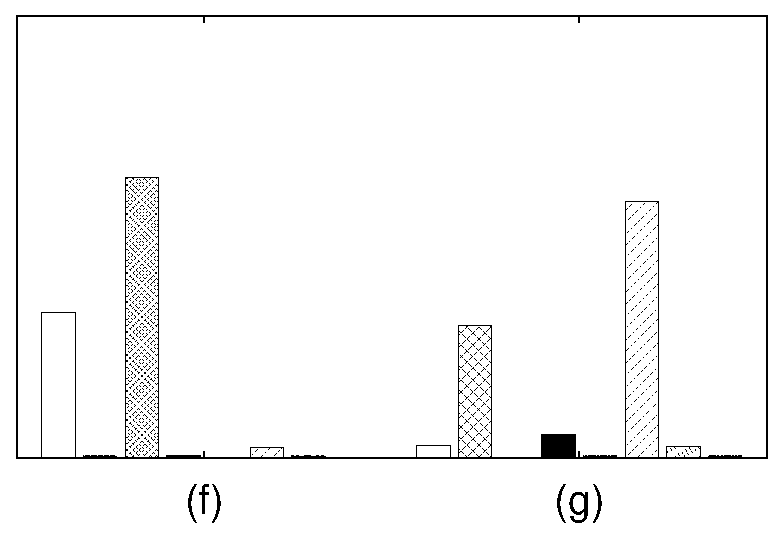
\epsfig{file=histogram2.eps, width=\columnwidth}
\end{minipage}
\hfill
\begin{minipage}[t]{0.295\columnwidth}
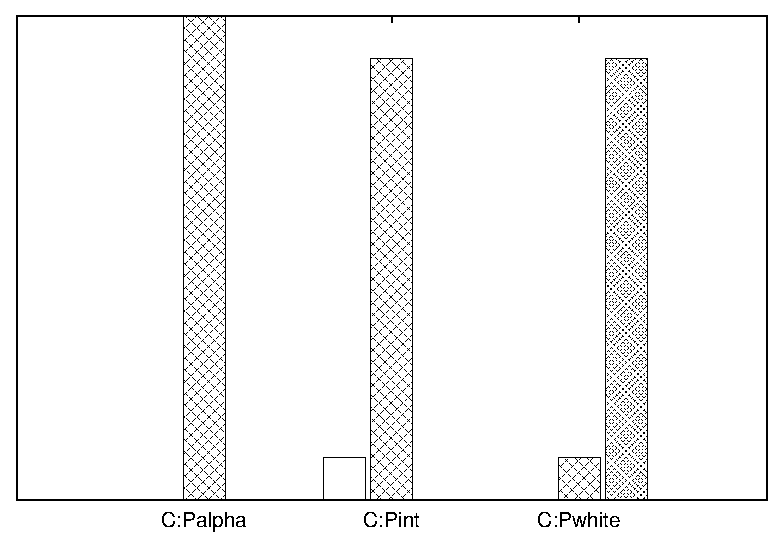
\epsfig{file=histogram3.eps, width=\columnwidth}
\end{minipage}
\hfill
\begin{minipage}[t]{0.59\columnwidth}
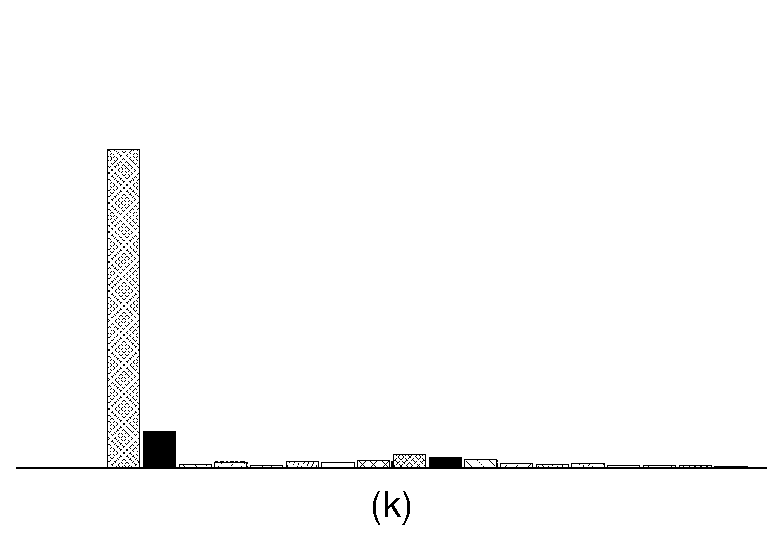
\epsfig{file=histogram4.eps, width=\columnwidth}
\end{minipage}
%
%a) histogram for ' '
%histogram for ':'
%...
%
%Omit telling the reader which histograms are for which tokens in the figure.
%We'll explain in the text...
%
%May 6 of them 3 each from Crashreporter.log and Sirius?
%We'll pick carefully.
\caption{Histograms (a), (b), (c), (d), (e), (f) and
(g) are generated from top-level analysis of Crashreporter.log tokens.
The corresponding tokens are (a) {\tt [*]}, 
(b)  {\tt Pint}, (c) {\tt PDate}, (d) {\tt PTime}, (e) {\tt -}, (f) {\tt Palpha} and
(g) {\tt Pwhite}.  Histograms (h) {\tt Palpha}, (i) {\tt Pint}, and 
(j) {\tt Pwhite} are generated from analysis of Crashreporter.log from
set 1 (the second level of recursion).  Histogram (k) is generated from
top-level analysis of the {\tt |} token from Dibbler.1000.}
\label{fig:histograms} 
\end{center}
\end{figure*}

As a first example, consider histogram (a)
from Figure~\ref{fig:histograms}.  This is the perfect candidate for a 
struct --
it has a single column that covers 100\% of the records.  Indeed,
this histogram corresponds to the \cd{[*]} token in Crashreporter.log.
Whenever such a histogram is detected, it will always be chosen
for immediate creation of a struct and partitioning.  All of the
other top-level histograms for Crashreporter.log contain variation
and hence are less certain indicators of data source structure.

As a second example, consider histograms (h), (i) and (j) and compare
them with histograms (f), (b) and (g). The histograms (h), (i) and (j)
are generated from the second level of recursive analysis. They
correspond to the histograms for chunk set 1, explained in the
previous subsection.  These histograms have far less variation in them
than the corresponding top-level histograms.  In particular, notice
that histogram (h) is a perfect struct histogram whereas histogram (f)
contains a great deal of variation.  This example illustrates where
the real power of our divide-and-conquer algorithm comes from -- if
{\em just one token} in the top-level structure can be identified as a
good partitioner for the data, it is very often the case that in the
next level of recursive analysis, the histograms become substantially
sharper and more amenable to analysis.

As a third example, consider histogram (k).  This histogram illustrates
the classic pattern for tokens involved in arrays -- it has a very long
tail.  And indeed, the \cd{|} token in the Dibber.1000
data does act like a separator for fields of an array.

To make the intuitions discussed above precise, we must define a number of
properties of histograms.  First, a histogram $h$ is a list of pairs
of natural numbers $(x,y)$ where $x$ denotes the token frequency and
$y$ denotes the number of records with that frequency.  
All first elements of pairs in the list must be unique.  
The {\em width} of a
histogram ({\em width}($h$)) is the number of elements in the list
excluding the zero-bar ({i.e.,} excluding element $(0,y)$).  
A histogram
$\normal{h}$ is in normal form when the first element of the list is
the zero column and all subsequent elements are sorted in descending
order by the $y$ component.  For example, if $h_1$ is the histogram
$[(0,5), (1,10), (2,25), (3,15)]$ then {\em width}($h_1$) is 3 and its
normal form $\normal{h_1}$ is $[(0,5), (2, 25), (3,15), (1,10)]$.

We often refer to $y$ as the {\em mass} of the element $(x,y)$
and given a histogram $h$, we refer to the mass of the $i^{\mathrm th}$
element of the list 
using the notation $h[i]$.  For instance, $h_1[3] = 15$ and 
$\normal{h_1}[3] = 10$.  The {\em residual mass} ({\em rm}) of a column $i$ in 
a normalized histogram $h$ is the mass of all the columns to the right of 
$i$ plus the mass of the zero-bar.  Mathematically, 
{\em rm}$(\normal{h},i) = \normal{h}[0] + \sum_{j=i+1}^{\mathit{width}(\normal{h})} \normal{h}[j]$.
For example, {\em rm}$(\normal{h_1},1) = 5 + 15 + 10 = 30$.
The residual mass is the primary characterization of ``narrowness''
of a histogram.  Those histograms with low residual mass of the first
column ({\em i.e.,} {\em rm}$(\normal{h_1},1)$ is small) 
are good candidates for structs.

In order to distinguishing between
structs, unions and arrays,
we also need to define the {\em coverage} of a histogram, which
is simply the sum of the non-zero histogram elements.  Mathematically,
{\em coverage}$(\normal{h}) = 
                  \sum_{j=1}^{\mathit{width}(\normal{h})} \normal{h}[j]$.

Finally, recursive partitioning of the data works better when
groups of tokens with similar distributions are considered together
-- when the algorithm has access to a sufficient amount of data and
two tokens have the same distribution, it is always the 
case that they form part of the same type constructor.  There are a 
number of ways to define {\em similarity} of histograms.  We have
chosen a symmetric form of {\em relative entropy} \cite{Lin91:divergence}.
%\footnote{Suggested by Rob Schapire, personal communication, May 2007.}  
The (plain) relative entropy
of two normalized histograms $\normal{h_1}$ and $\normal{h_2}$, 
written \relativee{\normal{h_1}}{\normal{h_2}}, is
defined as follows.
\[
 \relativee{\normal{h_1}}{\normal{h_2}} 
   = \sum_{j=1}^{\mathit{width}(\normal{h_1})} \normal{h_1}[j]*log(\normal{h_1}[j]/\normal{h_2}[j])
\]
To create a symmetric form, we first find the average of the two
histograms in question (written $\addh{h_1}{h_2}$)
by summing corresponding columns and dividing by two.  This
has the effect of preventing the denominator from being zero in the 
final relative entropy computation.  At last, the symmetric
relative entropy is:
\[
 \srelativee{\normal{h_1}}{\normal{h_2}} 
   = \frac{1}{2}  \relativee{\normal{h_1}}{\addh{\normal{h_1}}{\normal{h_2}}}
   +  \frac{1}{2}  \relativee{\normal{h_2}}{\addh{\normal{h_1}}{\normal{h_2}}}
\]

Now that we have defined the relevant properties of histograms,
we can explain how to guess type constructors.

\begin {enumerate}
\item Identify a base type when each chunk contains the same single token.

\item Otherwise, group related histograms into sets as follows.  
A histogram $h_1$ belongs to
group $G$ provided there exists another histogram $h_2$ in $G$
such that $\srelativee{\normal{h_1}}{\normal{h_2}} < 
\mathrm{ClusterTolerance}$.  We have found a ClusterTolerance
of 0.01 is effective.  A histogram dissimilar to all others may form 
its own group.

\item Identify a struct by 
considering all groups $G$, in descending order by residual mass
of the minimum histogram in the group.
The first group $G$ that contains any histograms $h$ that satisfy the
 following minimum criteria will be declared a struct on this 
iteration of the recursive algorithm:
\begin {itemize}
\item $\mathit{rm}(h) < \mathrm{MaxMass}$
\item $\mathit{coverage}(h) > \mathrm{MinCoverage}$
\end{itemize}
If no histograms satisfy the struct criterion, check for arrays.
If histograms $h_1$, $h_2$, {\em etc.} do satisfy the struct criterion, 
then partition the current chunks into subsequences separated
by tokens $t_1$, $t_2$, {\em etc.}  If tokens $t_1$, $t_2$, {\em etc.}
appear in different orders in different chunks, introduce a union of structs
instead of a simple struct, with one branch of the union per token 
ordering.  If some chunks do not contain the appropriate tokens, 
create a separate branch of the union for those chunks.

\item Identify an array by considering all groups $G$, in descending 
order by coverage of the highest coverage histogram in the group.
The first group $G$ that contains any histograms that satisfy the
 following minimum criteria will be declared an array on this 
iteration of the recursive algorithm:
\begin {itemize}
\item $\mathit{width}(h) > 3$
\item $\mathit{coverage}(h) > \mathrm{MinCoverage}$
\end{itemize}
If no tokens in any group satisfies the array criterion, find a union.
If histograms $h_1$, $h_2$, {\em etc.}, do satisfy the array criterion, 
then partition the current chunks into (1) a preamble subsequence 
that contains 1 occurrence of corresponding tokens $t_1$, $t_2$, {\em etc.},
(2) a set of element subsequences, with each subsequence containing
1 occurrence of the corresponding tokens  $t_1$, $t_2$, {\em etc.}, and
(3) a postamble subsequence that contains the last occurrence of 
the corresponding tokens $t_1$, $t_2$, {\em etc.}

\item Identify a union by partitioning the current set of chunks according
to the first token in each chunk.  Create one new set of chunks per first 
token.
\end{enumerate}

%%     *  role = quickly find a description in the "approximate area" of the correct description
%%     * explain structure of a generic "top-down" inference algorithm -- perhaps give pseudocode
%%     * explain our heuristics: generation of histograms, choice of struct, array, union, base type
%%     * grouping construct (introduce additional example as needed)
%%     * show (part of?) description of running example 

\subsection {Information-Theoretic Scoring}

The goal of the scoring function is to assess the quality of any
inferred description.  This quality metric guides decisions concerning
which rewriting rules to use to refine and transform a candidate
description, as explained in the following section.

Intuitively, a good description is one that is both {\em compact} and
yet {\em precise}.  There are trivial descriptions of any data source
that are highly compact ({\em e.g.,} the description that says
the data source is a string terminated by end of file) or
perfectly precise ({\em e.g.,} the data itself abstracts nothing and
therefore serves as its own description).  A good scoring function
carefully balances these two opposing constraints.  As is common
in machine learning, we have defined a scoring function based on the
{\em Minimum Description Length Principle} (MDL), which states that
a good description is one that minimizes the cost (in bits) of transmitting
the data.  This is accomplished by minimizing 
the sum of the cost of transmitting
the syntax of the description ($\costdescription{T}$)
plus the cost of transmitting the data 
relative to the information known given the description
($\costdata{T}{d_1,\ldots,d_k}$).  Mathematically,
if $T$ is a description and $d_1,\ldots,d_k$ are representations of
the $k$ chunks in our training set, parsed according to $T$, then the 
total cost in bits is:
\[
\totalcost{T}{d_1,\ldots,d_k} = \costdescription{T} + \costdata{T}{d_1,\ldots,d_k}
\]

%\paragraph*{The cost of transmitting a type.}
The cost of transmitting a type, measured in bits, is defined in 
Figure~\ref{fig:cost-type}.  In general, the cost of transmitting
a type is the cost of transmitting the sort of type ({\em i.e.,}\cd{struct},
\cd{union}, \cd{enum}, etc.) plus the cost of transmitting all subcomponents
of the type.  For example, the cost of transmitting any base type
$b(p_1,\ldots,p_k)$ is $ \cardt + \sum_{i=1}^{k} \costparam{p_i}$,
where $\cardt$ is the log of the number of different sorts of type 
constructors (24 of them in the \ir{} presented in this paper)
and $\costparam{p}$ is the cost of encoding the parameter $p$.
The cost of encoding variables, constants and parameters is not
shown in the figure, but is perfectly natural.  For instance, the cost of
encoding an ASCII character is 8 bits.  The cost of encoding a string
is the cost of encoding its length (assumed to be a 32-bit quantity)
plus the cost of encoding each character in turn.

The cost of encoding data relative to selected types is presented in 
Figure~\ref{fig:cost-data}.  At the top of the figure,
we present the cost of encoding all data
chunks relative to the type $T$; it is simply the sum of encoding
each individual chunk relative to $T$.  

In the middle of the figure,
we present the cost of encoding a chunk relative to one of the integer base 
types; other base types are handled similarly.  Notice that the cost of 
encoding an integer relative to the constant type \cd{PintConst} is
zero.  The reason is that the type itself contains all information
necessary to reconstruct the integer -- no data at all need be encoded.
The cost of encoding data relative to \cd{Pint32} or \cd{Pint64} types 
is simply 32 or 64 bits.  Finally, we artificially set the cost of
ranged types \cd{PintRanged}$(p_{min},p_{max})$ to be infinity.
Our experiments reveal that attempting to define integer types with
minimum and maximum values usually leads to overfitting of the data.
We nevertheless retain \cd{PintRanged} types in our \ir{} to encode
the range of values found during the value-space analysis.  During the
rewriting phase, this range information is used to rewrite \cd{PintRanged}
into other integer types.  Since the
cost of encoding \cd{PintRanged} is so high, the appropriate rewriting is 
guaranteed to be applied.  In the future, we may emit this range information
as comments in the generated descriptions.

The last section of Figure~\ref{fig:cost-data} presents the cost of
encoding data relative to selected type constructors.  For example,
the cost of encoding a \cd{struct} is the sum of the costs of encoding
it's component parts.  The cost of encoding a \cd{union} is the cost
of encoding the branch number ($log(k)$ if the union has $k$ branches)
plus the cost of encoding the branch itself.  The cost of encoding
an \cd{enum} is the cost of encoding it's tag only -- given the tag,
the underlying data is determined by the type.  The cost of encoding
a \cd{switch} is the cost of encoding the branch only -- the tag need not
be encoded because it is determined.

\begin{figure}
Miscellaneous definitions:
\[
\begin{array}{@{\,}l@{\,}c@{\,}l}
\cardt &=& \mbox{log of the number of type constructors in the \ir{}}
\end{array}
\]
Cost of transmitting constants and parameters:
\[
\begin {array} {@{}l@{\,}c@{\,}l}
\costchar{a}  &=& \mbox{Cost of transmitting character } a \\
\coststring{s}  &=& \mbox{Cost of transmitting string } s \\
\costint{i}  &=& \mbox{Cost of transmitting integer } i \\
\costconst{c}  &=& \mbox{Cost of transmitting constant } c \\
\costvar{x} &=& \mbox{Cost of transmitting variable } \\
\costparam{p}  &=& \mbox{Cost of transmitting parameter } p \\
\end{array}
\]
Cost of transmitting a type:
\[
\begin{array}{@{}l@{\,}c@{\,}l}
\costdescription{b(p_1,\ldots,p_k)} &=& 
  \cardt + \sum_{i=1}^{k} \costparam{p_i} \\
\costdescription{x{:}b(p_1,\ldots,p_k)} &=& 
  \cardt + \costvar{x} + \sum_{i=1}^{k} \costparam{p_i} \\
\costdescription{\mathtt{struct \{} T_1;\ldots ;T_k; \mathtt{\}}} &=& 
  \cardt + \sum_{i=1}^{k} \costdescription{T_i} \\
\costdescription{\mathtt{union \{} T_1; \ldots ;T_k; \mathtt{\}}} &=& 
  \cardt + \sum_{i=1}^{k} \costdescription{T_i} \\
\costdescription{\mathtt{enum \{} c_1,\ldots,c_k \mathtt{\}}} &=& 
  \cardt + \sum_{i=1}^{k} \costconst{c_i} \\
\end{array}
\]

\caption {Cost of transmitting a type, selected rules}
\label{fig:cost-type}
\end{figure}

\begin{figure}
Cost of encoding all training data relative to a type:
\[
\begin{array}{@{}lcl}
\costdata{T}{d_1,\ldots,d_k} &=& \sum_{i=1}^{k} \adc{T}{d_i} \\
\end{array}
\]
Cost of encoding a single chunk relative to selected base types:
\[
\begin{array}{@{}lcl}
\adc{\mathtt{PintConst}(p)}{i}      &=& 0 \\
\adc{\mathtt{Pint32}}{i}            &=& 32 \\
\adc{\mathtt{Pint64}}{i}            &=& 64 \\
\adc{\mathtt{PintRanged}(p_{min},p_{max})}{i} &=& \infty \\
\end{array}
\]
Cost of encoding a single chunk relative to selected types:

{\em needs more space in between definitions... cannot figure out how
to add it properly without another whole new line
in between definitions...}

\begin{tabbing}
XXXX\=XXXX\=\+\kill
$\adc{\mathtt{struct \{} T_1;\ldots T_k; \mathtt{\}}}{(d_1,\ldots,d_k)}$ \\
  \> $= \sum_{i=1}^{k} \adc{T_i}{d_i}$ \\ 
$\adc{\mathtt{union \{} T_1;\ldots T_k; \mathtt{\}}}{in_i(d)}$ \\            
  \> $= \mathtt{log}(k) + \adc{T_i}{d}$ \\
$\adc{\mathtt{enum \{} c_1;\ldots c_k; \mathtt{\}}}{in_i(c)}$ \\            
  \> $= \mathtt{log}(k)$ \vspace{3pt} \\
$\adc{
\mathtt{switch}\; x \; 
  \mathtt{of \{} 
    c_1 \mathtt{=>} T_1; \ldots  
    c_k \mathtt{=>} T_k; 
  \mathtt{\}}
}{in_i(d)}$ \\ 
  \> $= \adc{T_i}{d}$ \\
\end{tabbing}


\caption {Cost of transmitting data relative to a type, selected rules}
\label{fig:cost-data}
\end{figure}

\subsection {Structure Refinement}

%\documentclass[fleqn]{article}
\usepackage{code}
\newcommand{\struct}[1]{{\tt struct}\{#1\}}
\newcommand{\union}[1]{{\tt union}\{#1\}}
\newcommand{\enum}[1]{{\tt enum}\{#1\}}
\newcommand{\parray}[1]{{\tt array}\{#1\}}
\newcommand{\arrayFW}[2]{{\tt arrayFW}\{#1\}[#2]}
\newcommand{\switch}[2]{{\tt switch}(#1)\{#2\}}
\newcommand{\option}[1]{{\tt option}\{#1\}}
\newcommand{\goto}{\Rightarrow}
\begin{document}
\section{Rewriting Rules}
\subsection*{Data independent rules}
\begin{enumerate}
\item Singleton structs and unions.
\[
\struct{T} \goto T
\]
\[
\struct{} \goto \bot 
\]
\[
\union{T} \goto T
\]
\[
\union{} \goto \bot 
\]

\item Struct and union clean-up
\[
\struct{T_1; \ldots; T_i; \bot; T_j; \ldots; T_n} \goto
\struct{T_1; \ldots; T_i; T_j; \ldots; T_n} 
\] 
\[
\struct{T_1; \ldots; T_i; \emptyset; T_j; \ldots; T_n} \goto
\struct{T_1; \ldots; T_i; T_j; \ldots; T_n} 
\] 

\[
\union{T_1; \ldots; T_i; \bot; T_j; \ldots; T_n} \goto
\union{T_1; \ldots; T_i; T_j; \ldots; T_n} 
\] 
\[
\union{T_1; \ldots; T_i; \emptyset; T_j; \ldots; T_n} \goto
\union{T_1; \ldots; T_i; T_j; \ldots; T_n; \emptyset} 
\]
\noindent where $\emptyset$ means {\tt Pempty}.

\item Union to option
\[
\union{T; \emptyset} \goto \option{T}
\]
\[
\union{\emptyset; T} \goto \option{T}
\]

\item Unnest structs and unions
\begin{eqnarray*}
&& \struct{pretypes; \struct{T_1; \ldots; T_n}; posttypes} \goto \\
&& \struct{pretypes; T_1; \ldots; T_n; posttypes}
\end{eqnarray*}
\begin{eqnarray*}
&&\union{pretypes; \union{T_1; \ldots; T_n}; posttypes} \goto \\
&&\union{pretypes; T_1; \ldots; T_n; posttypes}
\end{eqnarray*}

\item Uniform struct to fixed-length array
\[
\struct{T_1; \ldots; T_n} \goto \arrayFW{T_1}{n}
\]
\noindent if $T_1 = \ldots = T_n$ and $n>=3$.

\item Common prefix or postfix in union branches
\begin{eqnarray*}
&&\union{\struct{T; posttypes_1}; \struct{T, posttypes_2}} \goto \\
&&\struct{T; \union{\struct{posttypes_1}; \struct{posttypes_2}}}
\end{eqnarray*}
\begin{eqnarray*}
&&\union{\struct{T; posttypes}; T} \goto \\
&&\struct{T; \union{\struct{posttypes}; \emptyset}}
\end{eqnarray*}
\begin{eqnarray*}
&&\union{\struct{pretypes_1; T}; \struct{pretypes_2; T}} \goto \\
&&\struct{\union{\struct{pretypes_1}; \struct{pretypes_2}}; T}
\end{eqnarray*}
\begin{eqnarray*}
&&\union{\struct{pretypes; T}; T} \goto \\
&&\struct{\union{\struct{pretypes}; \emptyset}; T}
\end{eqnarray*}

\item {Get floating number number}
\[
\union{{\tt Pint}; {\tt Pfloat}} \goto {\tt Pfloat}
\]

\end{enumerate}

\subsection*{Data dependent rules}
\begin{enumerate}
\item Get floating point number
\begin{eqnarray*}
&& \struct{pretypes; {\tt Pint}(x); {\tt PstringConst ('.')}; {\tt Pint}(y); posttypes} \goto \\
&& \struct{pretypes; {\tt Pfloat}; posttypes}
\end{eqnarray*}
\noindent if $y \ge 0$.
\begin{eqnarray*}
&& \struct{pretypes; {\tt Pint}(x); \option{\struct{{\tt PstringConst ('.')}; {\tt Pint}(y)}}; posttypes} \goto \\
&& \struct{pretypes; {\tt Pfloat}; posttypes}
\end{eqnarray*}
\noindent if $y \ge 0$.

\item Discover negative numbers
\begin{eqnarray*}
&& \struct{pretypes; {\tt Pother}; {\tt PstringConst}('-'); {\tt Pint}(x); posttypes} \goto \\
&& \struct{pretypes; {\tt Pother}; {\tt Pint}; posttypes}
\end{eqnarray*}
\noindent if $x \ge 0$.
\begin{eqnarray*}
&& \struct{pretypes; {\tt Pother}; {\tt PstringConst}('-'); {\tt Pfloat}(x); posttypes} \goto \\
&& \struct{pretypes; {\tt Pother}; {\tt Pfloat}; posttypes}
\end{eqnarray*}
\noindent if $x \ge 0$.
\begin{eqnarray*}
&& \struct{pretypes; {\tt Pother}; \option{{\tt PstringConst}('-')}; {\tt Pint}(x); posttypes} \goto \\
&& \struct{pretypes; {\tt Pother}; {\tt Pint}'; posttypes}
\end{eqnarray*}
\noindent if $x \ge 0$.
\begin{eqnarray*}
&& \struct{pretypes; {\tt Pother}; {\tt \option{PstringConst}('-')}; {\tt Pfloat}(x); posttypes} \goto \\
&& \struct{pretypes; {\tt Pother}; {\tt Pfloat}'; posttypes}
\end{eqnarray*}
\noindent if $x \ge 0$.

\item Unique base types to constant
\[
{\tt Pint}(x) \goto {\tt PintConst(c)}~~ {\rm if}~~ x = c.
\]
\[
{\tt Palpha}(x) \goto {\tt PstringConst(c)}~~ {\rm if}~~ x = c.
\]
\[
{\tt Pstring}(x) \goto {\tt PstringConst(c)}~~ {\rm if}~~ x = c.
\]
\[
{\tt Pother}(x) \goto {\tt PstringConst(c)}~~ {\rm if}~~ x = c.
\]


\item Combine adjacent constant strings
\begin{eqnarray*}
&& \struct{pretypes; {\tt PstringConst (c_1)}; {\tt PstringConst(c_2)}; posttypes} \goto \\
&& \struct{pretypes; {\tt PstringConst (c_1 + c_2)}; posttypes} 
\end{eqnarray*}

\item Refine enums and ranges
\[
{\tt Pstring}(x) \goto \enum{s_1; \ldots; s_k} ~~
{\rm if}~ x~ \in \{s_1, \ldots, s_l\}.
\]
\[
{\tt Pint}(x) \goto {\tt Pint32} ~~
{\rm if}~ 0 \le x~ < 2^{32}.
\]
\[
{\tt Pint}(x) \goto {\tt Pint64} ~~
{\rm if}~ 2^{32} \le x~ < 2^{64}.
\]

\[
{\tt Pint}(x) \goto {\tt PintRanged}(min,~ max) ~~
{\rm if}~ min \le x~ \le max.
\]
\item Union to switch
\begin{eqnarray*}
&&\struct{pretypes; b(x); midtypes; \union{T_1; \ldots; T_n}; posttypes} \goto \\
&&\struct{pretypes, b(x); midtypes; \switch{x}{s_1 \goto T_1; \ldots; s_n \goto T_n}; posttypes}
\end{eqnarray*}
\noindent where $\forall i \in [i,~ n],~ inj_i(\union{T_1; \ldots; T_n}) {\rm implies}~ x = s_i$.

\end{enumerate}

\end{document}


%    *  role = starting with the candidate structure, search for nearby descriptions that optimize an information theoretic scoring function
%    * explain the 3 parts: value independent, value dependent, value independent
%    * give (partial) list of rules used -- we need to work on notation for explaining these rules
%    * illustrate several transformations using the running example
%    * compare example after rewriting to the example from subsection 3.4 above
%    * optional subsubsection: theory suggesting our algorithm is "correct" (we'd need a semantics for our IR then)

The purpose of the structure refinement phase is to improve
the candidate structure produced by the structure discovery phase. We
formulate the structure refinement problem as a generalized search
through description space starting with the candidate produced by
structure discovery. The
objective of the search is to find the description that minimizes
the information-theoretic scoring function.

\paragraph*{Rewriting rules}
In order to move around in description space, we define a number of 
description rewriting rules. The general form of the rule is
\[T \goto T', ~~ {\rm if~ some~ constraint~} p(T)~ {\rm is~ satisfied,}\]
where $T$ is a type, or sub-structure, and $T'$ is the type after the
transition.  Some rules are unconditional and thus free of constraints.
There are two kinds of rewriting rules: (1) data-independent rules which
transform a type based exclusively on the syntax of the description; 
and (2) data-dependent
rules which transform a type based on both the syntax of the description
and on properties of the training data
parsed by this type.  In general, 
the data independent rules aim to rearrange and merge portions
of the structure while the data dependent rules seek to identify 
constant fields and enumerations, and to establish relationships 
between different parts of the structure.

In Figure \ref{fig:rules}, we present a selection of the
data independent and data dependent rules used in the refinement phase.
Many rules have been omitted and some have been simplified for succinctness.
%In these rules,
%let $T_{punc}$ be any type that describes punctuation or white space character%s.
When $T\setof{X}$ appears in a pattern on the left-hand side of a rewriting
rule, $X$ is bound to the set of data representations resulting
from using $T$ to parse the appropriate part of each chunk from the training
set. Furthermore, let $card(X)$ be the cardinality of the set $X$, 
and let $X(i)$ be the data representation resulting
from parsing the $i^{th}$ chunk in the training set. Finally, given a union
value $\mathtt{in}_j(v)$, we define $tag(\mathtt{in}_j(v))$ to be $j$.

\begin{figure*}
\begin{center}
\framebox{
\noindent
\begin{minipage}[t]{\columnwidth}
\paragraph*{Data independent rules}
\begin{enumerate}
\item Singleton structs and unions \\
$
\irstruct{T} \goto T  \qquad\qquad\quad \irunion{T} \goto T
$\\ \\
$
\irstruct{} \goto \Pempty  \qquad\quad\quad \irunion{} \goto \Pvoid 
$
\item Struct and union clean-up\\
$
\irstruct{pre\_types; \Pvoid; post\_types} \goto \Pvoid
$\\ \\ 
$
\irstruct{pre\_types; \Pempty; post\_types} \goto \\
\sskip \irstruct{pre\_types; post\_types}
$\\ \\ 
$
\irunion{pre\_types; \Pvoid; post\_types} \goto \\
\sskip \irunion{pre\_types; post\_types} 
$
%$
%\irunion{pre\_types; \Pempty; post\_types} \goto \\
%\sskip \irunion{pre\_types; post\_types; \Pempty} 
%$
% \item Union to option\\
% $
% \irunion{T; \Pempty} \goto \iroption{T}
% $\\ \\
% $
% \irunion{\Pempty; T} \goto \iroption{T}
% $
% \item Unnest structs and unions\\
% $
% \irstruct{pre\_types; \irstruct{mid\_types}; post\_types} \goto \\
% \sskip \irstruct{pre\_types; mid\_types; post\_types}
% $\\ \\
% $
% \irunion{pre\_types; \irunion{mid\_types}; post\_types} \goto \\
% \sskip \irunion{pre\_types; mid\_types; post\_types}
% $
\item Uniform struct to fixed-length array\\
$
\irstruct{T_1; \ldots; T_n} \goto \irarrayFW{T_1}{n}
$\\ 
\noindent if $n \ge 3$ and $\forall i \in [1,~ n],~ j \in [1,~ n]:~ T_i = T_j$.

\item Common postfix in union branches \\
% $
% \irunion{\irstruct{T; post\_types_1}; \\
% \sskip \irstruct{T, post\_types_2}} \goto \\
% \sskip \irstruct{T; \irunion{\irstruct{post\_types_1}; \\
% \sskip \irstruct{post\_types_2}}}
% $\\ \\
% $
% \irunion{\irstruct{T; post\_types}; T} \goto\\
% \sskip \irstruct{T; \iroption{\irstruct{post\_types}}}
% $\\ \\
$
\irunion{\irstruct{pre\_types_1; T}; \\
\sskip \irstruct{pre\_types_2; T}} \goto \\
\sskip \irstruct{\irunion{\irstruct{pre\_types_1}; \\
\sskip \irstruct{pre\_types_2}}; T}
$\\ \\
$
\irunion{\irstruct{pre\_types; T}; T} \goto \\
\sskip \irstruct{\iroption{\irstruct{pre\_types}}; T}
$

\item Combine adjacent constant strings \\
$
\irstruct{pre\_types; {\tt PstringConst (c_1)}; \\
\sskip {\tt PstringConst(c_2)}; post\_types} \goto \\
\sskip \irstruct{pre\_types; {\tt PstringConst (c_1 {\makeatletter \tt @} c_2)}; post\_types} 
$

% \item {Get floating number number}\\
% $
% \irunion{{\tt Pint}; {\tt Pfloat}} \goto {\tt Pfloat}
% $ 

\end{enumerate}
\end{minipage}
\hfill
\begin{minipage}[t]{\columnwidth}
\paragraph*{Data dependent rules}
\begin{enumerate}
% \item Get floating point number \\
% $
% \irstruct{pre\_types; {\tt Pint}\setof{X}; {\tt PstringConst ('.')};  \\
% \sskip {\tt Pint}\setof{Y}; post\_types} \goto \\
% \sskip \irstruct{pre\_types; {\tt Pfloat}; post\_types}
% $\\ 
% \noindent if $\forall y \in Y:~ y \ge 0$. \\
% \\
% $
% \irstruct{pre\_types; {\tt Pint}\setof{X}; \\
% \sskip \iroption{\irstruct{{\tt PstringConst ('.')};  \\
% \sskip {\tt Pint}\setof{Y}}}; post\_types} \goto \\
% \sskip \irstruct{pre\_types; {\tt Pfloat}; post\_types}
% $ \\
% \noindent if $\forall y \in Y:~ y \ge 0$. 

% \item Discover negative numbers\\
% $
% \irstruct{pre\_types; T_{punc}; {\tt PstringConst}('-');\\
% \sskip {\tt Pint} \setof{X}; post\_types} \goto \\
% \sskip \irstruct{pre\_types; T_{punc}; {\tt Pint}; post\_types}
% $\\ 
% \noindent if $\forall x \in X:~ x \ge 0$. \\
% \\
% $
%  \irstruct{pre\_types; T_{punc}; {\tt PstringConst}('-'); \\
% \sskip {\tt Pfloat}\setof{X}; post\_types} \goto \\
% \sskip \irstruct{pre\_types; T_{punc}; {\tt Pfloat}; post\_types}
% $\\ 
% \noindent if $\forall x \in X:~ x \ge 0$.\\
% \\
% $
%  \irstruct{pre\_types; T_{punc}; \iroption{{\tt PstringConst}('-')}; \\
% \sskip {\tt Pint}(x); post\_types} \goto \\
% \sskip \irstruct{pre\_types; T_{punc}; {\tt Pnat}; post\_types}
% $\\
% \noindent if $\forall x \in X:~ x \ge 0$.\\
% \\
% $
% \irstruct{pre\_types; T_{punc}; {\tt \iroption{PstringConst}('-')}; \\
% \sskip {\tt Pfloat}(x); post\_types} \goto \\
% \sskip  \irstruct{pre\_types; T_{punc}; {\tt Preal}; post\_types}
% $\\
% \noindent if $\forall x \in X:~ x \ge 0$.

\item Base type with unique values to constant \\
$
{\tt Pint}\setof{X} \goto {\tt PintConst(c)} \\
$
{\rm if} $\forall x \in X:~ x = c$. 
\\ \\
$
{\tt Palpha}\setof{X} \goto {\tt PstringConst(c)} \\
$
{\rm if} $\forall x \in X:~ x = c$.
\\ \\
$
{\tt Pstring}\setof{X} \goto {\tt PstringConst(c)} \\
$
{\rm if} $\forall x \in X:~ x = c$.
\\ \\
$
{\tt Pother}\setof{X} \goto {\tt PstringConst(c)} \\ 
$
{\rm if} $\forall x \in X:~ x = c$.

\item Refine enums and ranges \\
$
{\tt Pstring}\setof{X} \goto \irenum{s_1; \ldots; s_k} \\
$
{\rm if}~ $\forall x \in X:~ x~ \in \{s_1, \ldots, s_k\}$.
\\ \\
$
{\tt Pint}\setof{X} \goto {\tt Pint32} \\
$
{\rm if} $\forall x \in X:~ 0 \le x~ < 2^{32}$.
% $
% {\tt Pint}\setof{X} \goto {\tt Pint64} \\
% $
% {\rm if} $\forall x \in X:~ 2^{32} \le x~ < 2^{64}$.
% \\ \\
% $
% {\tt Pint}\setof{X} \goto {\tt PintRanged}(min,~ max) \\
% $
% {\rm if}~ $\forall x \in X:~ min \le x~ \le max$.

\item Union to switch \\
$
\irstruct{pre\_types; \irenum{c_1; \ldots; c_n}\setof{X}; mid\_types; \\
\sskip \irunion{T_1; \ldots; T_n}\setof{Y}; post\_types}\\
\goto \\
\irstruct{pre\_types, z:\irenum{c_1; \ldots; c_n}; mid\_types; \\
\sskip \irswitch{z}{c_1 \goto T_{\Pi(1)}; \ldots; c_n \goto T_{\Pi(n)}}; post\_types}
$\\ 
\noindent where $z$ is a fresh variable, and there exists a permutation $\Pi$, s.t.  $\forall i \in [1,~ card(X)]$, $\Pi(tag(X(i)))=tag(Y(i))$.
\end{enumerate}
\end{minipage}
}
\end{center}
\caption{Selected and simplified rewriting rules} \label{fig:rules}
\end{figure*}

\paragraph*{The Search.}
The core of the rewriting system is 
a recursive, depth-first, greedy search procedure. 
By ``depth-first,'' we mean the algorithm begins by refining the 
children of any structured type before
the structure itself. When refining a type, it selects a rule that 
would {\em minimize} the information-theoretic score of the resulting
structure and applies it to the structure.  It iterates this process until
no further reduction in the score is possible, and at
that time, structure $T$ is said to be {\em stable}.

\begin{figure}
{\small 
\begin{verbatim}
(* a rewriting rule *)
type rule : description -> description  

(* all relevant rules in a list *)
val rules : rule list 

(* measure the score for a type *)
fun score : description -> float

(* find the type with best score from a list *)
fun best: description list -> description

(* improve the given type by one rewriting rule *)
fun oneStep (T:description) : description =
 let all = map (fn rule => rule T) rules in
 let top = best all                      in
 if (score top) < (score T) then
   oneStep top
 else
   T

(* main function to refine an IR description *) 
fun refine (T:description) : description =
  let T' = case T of
      base b => b
    | struct { Ts } => struct { map refine Ts }
    | union { Ts } => union { map refine Ts }
    | switch x of { vTs } => 
       switch x of 
         { map (fn (v, t) => (v, refine t)) vTs }
    | array { T } => 
              array { refine T }
    | option { T } => option { refine T } in
  oneStep T'
\end{verbatim}
}
\caption{Generic local optimization algorithm in Pseudo-ML}
\label{fig:refinement}
\end{figure}

The overall algorithm in Figure \ref{fig:refinement} is applied three
times in succession. 
The first time, the algorithm quickly reduces the initial structure to 
a much simpler, more manageably-sized structure by using
the data-independent rules {\em only}. The second time, data dependent
rules are used refine the base types to constant values and enumerations, etc,
and establish structural dependencies such as switched unions. This phase
requires the value-space analysis described below.
The third time, the set of the data-independent rules
are applied again. The third time is necessary because certain changes
to the base types in phase two, such as the creation of constants, may 
newly enable some of the data-independent rules. 

\paragraph*{Value-space analysis.}
A value-space analysis is performed prior
to applying the data-dependent rules.
This analysis operates by first generating a set of relational tables
from the input data.
Each row of a table corresponds to a chunk and each column of a table
corresponds to either a particular base type from the inferred description,
or to a piece of metadata from the description.  Examples of meta-data
include the tag number from union branches and the length of arrays.
We generate a {\em set} of relational tables as opposed to a single table
as the elements of an array occupy their own separate table (a description 
with no arrays will only have one associated table).
% Here, a number of data dependency tables are generated from the 
% input structure, where each
% column of the tables represent the data values associated with a particular base type 
% in the structure, with some extra columns representing auxilliary information such as
% array sizes and union branching decisions.
 
Every column of every table is analyzed to determine properties,
such as constancy and value range, of the data in that column.
To determine inter-column properties, we have implemented a simplified
variant of the TANE algorithm \cite{TANE-HKPT99},
which identifies functional dependencies between columns in 
relational data.  Because full TANE is too expensive 
(possibly exponential in the number of columns), 
and with insufficient data results in many false positives, 
our simplified algorithm only computes binary dependencies. The 
result of this dependency analysis is used to 
identify switched unions and fixed-size arrays.
%In addition, we also discover all the unary constraints on the base types by
%analysizing every single column in the data tables. We store these unary and
%binary constraint in a constraint map.  A rule can be applied 
%only if the conditions are validated successfully
%against the constraint map. 

\paragraph*{Running example}
To illustrate the refinement process a bit more concretely, let us walk through
a few steps as the system refines the initial structure of the crashreporter.log example.
Let us zoom into the beginning portion of the IR and omit some of the details as follows. 
We annotate each type with two pieces of auxiliary information: id of the node which
can be used as the variable name and the complexity score at this node, 
enclosed in a pair of parenthese. In addition, for Pother base types,
we append the character it binds to in parenthese after the type name.
The intial IR structure of crash reporter looks like this:

{\small
\begin{verbatim}
struct {
  union {
    struct {
      Pdate; Pwhite; Ptime; Pwhite; Pint;  
      Pwhite;          (*)
    };
    struct { 
      "-"; 
      Pwhite;          (*)
    };
  }
  Palpha; "["; Pint; "]";
  union { ... };
};
\end{verbatim}
}


% {\small
% \begin{verbatim}
% struct(BTy_114, 416156.763b) {
%   union(BTy_7, 204984.986b) {
%     struct(BTy_6, 204589.179b) {
%       Pdate (BTy_0, 108004.535b);
%       Pwhite (BTy_1, 809.044b);
%       Ptime (BTy_2, 88802.177b);
%       Pwhite (BTy_3, 809.044b);
%       Pint (BTy_4, 5347.705b);
%       Pwhite (BTy_5, 809.044b);
%     };
%     struct(BTy_10, 388.762b) {
%       Pother (-) (BTy_8, 299.673b);
%       Pwhite (BTy_9, 83.044b);
%     };
%   }
%   Palpha (BTy_11, 23879.044b);
%   Pother ([) (BTy_13, 3336.618b);
%   Pint (BTy_14, 6899.045b);
%   Pother (]) (BTy_15, 3336.618b);
%   union(BTy_63, 173712.822b) {
%     struct(BTy_62, 156487.759b) {
%       ...
%     };
%     struct(BTy_113, 17218.019b) {
%       ...
%     };
%   };
% };
% \end{verbatim}
% }

% {\small
% \begin{verbatim}
% struct(BTy_114, 416156.509b) {
%   struct(BTy_115, 204984.732b) {
%     union(BTy_7, 204091.634b) {
%       struct(BTy_6, 203779.872b) {
%         Pdate (BTy_0, 108004.535b);
%         Pwhite (BTy_1, 809.044b);
%         Ptime (BTy_2, 88802.177b);
%         Pwhite (BTy_3, 809.044b);
%         Pint (BTy_4, 5347.705b);
%       };
%       struct(BTy_10, 304.718b) {
%         Pother (-) (BTy_8, 299.673b);
%       };
%     }
%     Pwhite (BTy_5, 887.044b);
%   }
%   ...
% };
% \end{verbatim}
% }

% Note that we end up with an undesirable situation in BTy\_10 where a struct 
% contains just one element. That will be fixed in Phase three as we shall see.
% Next, the "unnest struct and union" rule kicks in to flatten struct BTy\_114 to
% the following.

In the first, value-independent phase of rewriting, 
the common trailing white space marked {\tt (*) } above is
pulled out of the unions and flattened inside the surrounding
struct using the ``common postfix in union'' rule.  This 
transformation leaves behind the unnecessarily verbose
single-element struct on the line marked {\tt (**)}.  However, this
will be transformed into the more compact constant 
string {\tt "-"} in phase three of rewriting.  This rewriting
phase also pulls colon and whitespace characters out of the 
trailing union (marked {\tt (**)}).

{\small
\begin{verbatim}
struct {
  union {
    struct { Pdate; Pwhite; Ptime; Pwhite; Pint; };
    struct { "-" };                 (**)
  }
  Pwhite;                           (*)
  Palpha; "["; Pint; "]"; ":"; Pwhite; (***)
  union { ... };
};
\end{verbatim}
}

% struct(BTy_114, 416056.899b) {
%     union(BTy_7, 204091.634b) {
%       struct(BTy_6, 203779.872b) {
%         Pdate (BTy_0, 108004.535b);
%         Pwhite (BTy_1, 809.044b);
%         Ptime (BTy_2, 88802.177b);
%         Pwhite (BTy_3, 809.044b);
%         Pint (BTy_4, 5347.705b);
%       };
%       struct(BTy_10, 304.718b) {
%         Pother (-) (BTy_8, 299.673b);
%       };
%     Pwhite (BTy_5, 887.044b);
%     ...
%   }
%   ...
% };

In the second rewriting phase, 
data-dependent rules 3 and 4 are applied to base types to 
create a number of constants and enums.
Moreover, a data dependency is discovered between the
newly introduced enumeration involving {\tt "crashdump"},
{\tt "mach\_msg"}, {\em etc.}, and the structure of the following message.
Hence, a switched union is also introduced.
Notice that the switched union is switching on a different enum 
than the hand-written IR in Figure \ref{fig:crashreporter:ir}, because
the inference algorithm has decided on a different way of partitioning
the chunks. Nonetheless, both of these descriptions are
correct.


{\small
\begin{verbatim}
struct {
  union {
    struct { Pdate; " "; Ptime; " "; 2006; };
    struct { "-" };
  };
  " "; enum {"crashreporterd", "crashdump"};
  "["; PintRanged [120...29874]; "]"; ":"; " ";
  x19:enum {"crashdump", "mach_msg", "Finished", 
            "Started", "Unable", "Failed"};
  switch x19 of { ... };
};
\end{verbatim}
}

% struct(BTy_114, 304553.986b) {
%   union(BTy_7, 196876.315b) {
%     struct(BTy_6, 196853.182b) {
%       Pdate (BTy_0, 108004.535b);
%       " " (BTy_1, 11.044b);
%       Ptime (BTy_2, 88802.177b);
%       " " (BTy_3, 11.044b);
%       2006 (BTy_4, 17.015b);
%     };
%     struct(BTy_10 39, 16.089b) {
%       "-" (BTy_8 39, 11.044b);
%     };
%   };
%   " " (BTy_5, 11.044b);
%   enum {"crashreporterd", "crashdump"}(BTy_11, 156.133b);
%   "[" (BTy_13, 11.044b);
%   Pint [120...29874] (BTy_14, 6580.450b);
%   "]" (BTy_10, 11.044b);
%   ":" (BTy_12, 11.044b);
%   " " (BTy_13, 11.044b);
%   enum {"crashdump", "mach_msg", "Finished", "Started", 
%         "Unable", "Failed"} (BTy_19, 317.405b);
%   union(BTy_63, 100570.505b) {
%     ...
%   };
% };


% Further, data dependency is discovered between type BTy\_19
% and the union BTy\_63, and thus the latter is converted to
% a switched union as follows.

% {\small
% \begin{verbatim}
% struct(BTy_114, 304552.986b) {
%   ...
%   enum {"crashdump", "mach_msg", "Finished", "Started", 
%         "Unable", "Failed"} (BTy_19, 317.405b);
%   switch BTy_14 of (BTy_63, 100569.505b) {
%     enum {"Failed", "Finished", "Started"}   => 
%       struct(BTy_57, 99696.280b) {
%        ...
%       };
%     enum {"Unable", "crashdump", "mach_msg"} =>
%       struct(BTy_108, 867.181b) {
%        ...
%       };
%   };
% };
% \end{verbatim}
% }

In the third and final phase, 
data independent rule 5  is applied to combine many constants 
and rule 1 is used to flatten the singleton struct. The final IR follows.

{\small
\begin{verbatim}
struct {
  union {
    struct { Pdate; " "; Ptime; " "; 2006; };
    "-";
  };
  " "; enum {"crashreporterd", "crashdump"};
  "["; Pint32; "]: ";
  x19:enum {"crashdump", "mach_msg", "Finished", 
        "Started", "Unable", "Failed"};
  switch x19 of { ... };
  };
};
\end{verbatim}
}


% {\small
% \begin{verbatim}
% struct(BTy_114, 304537.855b) {
%   union(BTy_7, 196876.315b) {
%     struct(BTy_6, 196853.182b) {
%       Pdate (BTy_0, 108004.535b);
%       " " (BTy_1, 11.044b);
%       Ptime (BTy_2, 88802.177b);
%       " " (BTy_3, 11.044b);
%       2006 (BTy_4, 17.015b);
%     };
%     "-" (BTy_8 39, 11.044b);
%   };
%   " " (BTy_5, 11.044b);
%   enum {"crashreporterd", "crashdump"}(BTy_11, 156.133b);
%   "[" (BTy_13, 11.044b);
%   Pint [120...29874] (BTy_14, 6580.450b);
%   "]: " (BTy_10, 23.044b);
%   enum {"crashdump", "mach_msg", "Finished", "Started", 
%         "Unable", "Failed"} (BTy_19, 317.405b);
%   switch BTy_14 of (BTy_63, 100569.505b) {
%     enum {"Failed", "Finished", "Started"}   => 
%       struct(BTy_57, 99696.280b) {
%        ...
%       };
%     enum {"Unable", "crashdump", "mach_msg"} =>
%       struct(BTy_108, 867.181b) {
%        ...
%       };
%   };
% };
% \end{verbatim}
% }

Comparing this final result with the initial description, one can see that
the structure refinement significately simplified the IR and improved the
complexity score; and with
the explicit constants and enums, the description is a lot more
informative than before.
 

\subsection {Final Products}

show part of pads syntax of inferred crashreporter as
well as xml data + gnuplot.
